%\chapter{Challenge 3: Duckie Detection}
%\chaptermark{Duckie Detection}
%\label{ch:DuckieDetection}

\section{Anforderungen und Herausforderungen}
\sectionmark{Anf}

Die zentrale Anforderung dieser Challenge bestand in der zuverlässigen Erkennung von statischen Objekten (Spielzeugenten) auf der Fahrbahn und der darauf aufbauenden Durchführung eines sicheren Ausweichmanövers. Die Implementierung musste gewährleisten, dass der Duckiebot einerseits präzise Hindernisse erkennt und lokalisiert, andererseits jedoch auch dynamisch auf neue Situationen reagieren kann – beispielsweise bei mehrfachen Enten oder einer verdeckten Sicht.

Ein wesentliches Ziel war die Reduktion von Fehlalarmen, etwa durch temporäre Bildartefakte oder unvollständige Objekterkennung. Zur Erhöhung der Robustheit wurde eine Mittelwertbildung über mehrere Frames implementiert. Hierbei flossen nur Objekte in die Entscheidungslogik ein, die mit einer definierten Wahrscheinlichkeit über die letzten zehn Bilder hinweg detektiert wurden.

Eine weitere Herausforderung ergab sich aus der Kombination von visueller Spurverfolgung und gleichzeitiger Trajektorienanpassung. Die Ausweichbewegung sollte nicht abrupt, sondern flüssig und zeitlich gesteuert erfolgen, um ein realistisches Fahrverhalten zu simulieren und die Regelung zu entlasten. Gleichzeitig musste sichergestellt sein, dass nach dem Ausweichen eine Rückführung auf die reguläre Spur erfolgt, ohne dabei erneut ein Hindernis zu treffen.

Schwierig gestaltete sich zudem die Handhabung inkonsistenter Sensorinformationen. Beispielsweise konnten sich erkannte Bounding Boxes kurzzeitig auflösen, was ohne geeignete Zwischenspeicherung zu einem ungewollten Abbruch des Ausweichvorgangs geführt hätte. Diese Problematik wurde durch ein Zeitfensterkonzept entschärft, das frühere Detektionen für eine kurze Zeitspanne als gültig speicherte und somit kurzfristige Erkennungsverluste tolerierte.

\section{Ablaufdiagramm}
\sectionmark{Impl}

Der Ablauf der Hindernisvermeidung ist in Abbildung~\ref{fig:duckie_avoidance_flow} schematisch dargestellt. Der Prozess beginnt im Status 0, in dem kontinuierlich geprüft wird, ob ein Duckie erkannt wird. Bei einer positiven Detektion wird über die untere Kante der Bounding Box ($y_2$) die Entfernung abgeschätzt. Liegt diese über einem definierten Schwellwert, erfolgt lediglich eine Reduktion der Geschwindigkeit (Info = 1), während bei Unterschreitung in den Status 1 gewechselt wird.

Im Status 1 beginnt das eigentliche Ausweichmanöver. Hierbei wird auf Basis der rechten Fahrspurmarkierung und einer Kosinusfunktion ein zeitlich gesteuerter Versatz berechnet, der die Querbewegung auf die linke Fahrbahnseite einleitet. Solange im rechten Sichtfeld noch Enten erkannt werden, bleibt der Duckiebot im Ausweichmodus.

Erst wenn über eine definierte Zeitspanne keine Objekte mehr auf der rechten Spur erkannt werden, wird in Modus 2 übergegangen. Dieser berechnet ein Rückführungsverhalten mit umgekehrter Kosinusbewegung, das die Rückkehr auf die rechte Spur einleitet. Nach erfolgreicher Rückführung wird der Zustand zurückgesetzt und der Zyklus beginnt von vorn.

\begin{figure}[htbp]
    \centering
    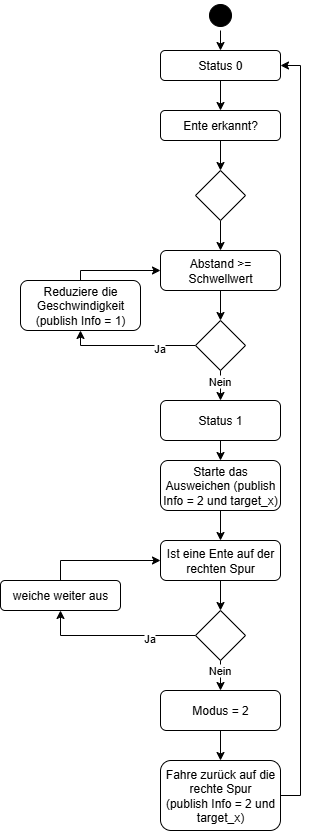
\includegraphics[width=0.6\textwidth]{Figures/png/Ablaufdiagramme_Bericht-Ausweichen.drawio.png}
    \caption{Ablaufdiagramm des Ausweichverhaltens}
    \label{fig:duckie_avoidance_flow}
\end{figure}

Die Kommunikation mit der \texttt{switch\_control\_node} erfolgt durch Veröffentlichung des Statuswerts über \texttt{/detect/duckie/info} sowie durch Publikation eines alternativen Zielpunkts \texttt{target\_x} auf \texttt{/detect/duckie/bypass\_target}. Die zentrale Steuerung entscheidet dann, ob dieser Wert priorisiert in die Regelung übernommen wird.


\section{Technische Umsetzung im Code}
\label{sec:Duckie_Code}

Die technische Umsetzung der Hinderniserkennung und des Ausweichverhaltens erfolgt über das Zusammenspiel zweier spezialisierter Nodes: der \texttt{detect\_object\_node} zur visuellen Objekterkennung mittels neuronaler Netze sowie der \texttt{bypass\_duckie\_node} zur Umsetzung eines zeitlich und geometrisch gesteuerten Ausweichmanövers (siehe Anhang, Listing~\ref{lst:detect_object_node} und Listing~\ref{lst:bypass_duckie_node}).

\subsection{Objekterkennung mit YOLOv8n}
Die \texttt{detect\_object\_node} basiert auf einem vortrainierten YOLOv8n-Modell, das in Echtzeit Objekte im Kamerabild klassifiziert. Erkannt werden insbesondere:
\begin{itemize}
    \item \texttt{Duckie} – kleine gelbe Hindernisse auf der Fahrspur
    \item \texttt{Bot} – andere Duckiebots
    \item \texttt{freeSlot} / \texttt{occupiedSlot} – Parkplätze
\end{itemize}

Jedes erkannte Objekt wird durch ein Bounding Box definiert und im Bild verortet. Die Zuverlässigkeit der Erkennung wird über eine Kombination aus Konfidenzschwellen und zeitlicher Mittelung (Moving Average) gesteigert. Zusätzlich wird über sogenannte Masken (vordefinierte Polygone) bestimmt, ob ein Objekt innerhalb eines relevanten Bereichs liegt – z.\,B. in der eigenen Spur oder im rechten Randbereich.

\newpage

Zur Ausgabe werden die ermittelten Bounding Boxes in \texttt{Float64MultiArray}-Nachrichten über dedizierte Topics veröffentlicht, u.\,a.:
\begin{itemize}
    \item \texttt{/detect/object/duckieNearestBB}
    \item \texttt{/detect/object/duckieNearestRightBB}
\end{itemize}
Diese Daten bilden die Grundlage für die Ausweichentscheidung in der nachfolgenden Node.

\subsection{Ausweichlogik in der Bypass-Node}
Die \texttt{bypass\_duckie\_node} verarbeitet die erkannte Position der Enten (v.\,a.\ das untere Ende der Bounding Box $y_2$), um ein phasenbasiertes Ausweichmanöver zu steuern. Das Verhalten ist in drei Modi unterteilt:

\begin{itemize}
    \item \textbf{Modus 0 – Normalfahrt:} Solange keine Ente erkannt wird oder diese weit entfernt ist ($y_2 < \texttt{min\_distance}$), erfolgt reguläre Spurverfolgung. Wird eine Ente als nah klassifiziert, wird in den Ausweichmodus gewechselt.
    
    \item \textbf{Modus 1 – Ausweichen:} Der Duckiebot führt eine schwenkförmige Bewegung zur Seite durch. Diese erfolgt durch eine zeitbasierte Offset-Berechnung über eine Kosinusfunktion:
    \begin{equation}
        \texttt{offset} = \cos\left( \frac{t}{T} \cdot \pi \right) \cdot \texttt{Amplitude}
    \end{equation}
    wobei $T$ die Dauer des Ausweichvorgangs und \texttt{Amplitude} der maximale seitliche Versatz ist. Der berechnete Zielpunkt \texttt{target\_x} wird auf das Topic \texttt{/detect/duckie/bypass\_target} publiziert.

    \item \textbf{Modus 2 – Rückkehr:} Nach Verlassen des Kollisionsbereichs (Ente rechts nicht mehr sichtbar) wird über eine gespiegelte Bewegung zurück auf die Ausgangsspur gelenkt. Nach Abschluss kehrt die Node in Modus~0 zurück.
\end{itemize}

Parallel zur Zielpunkt-Berechnung veröffentlicht die Node kontinuierlich einen Statuscode auf \texttt{/detect/duckie/info}:
\begin{itemize}
    \item 0: keine Ente erkannt
    \item 1: abbremsen (Ente fern)
    \item 2: aktiv ausweichen (Ente nah)
\end{itemize}

Dieser Code wird von der \texttt{switch\_control\_node} ausgewertet und beeinflusst die Auswahl des zu übergebenden \texttt{target\_x}-Wertes an die Regelung.

\subsection{Visualisierung und Debug}
Sowohl die \texttt{detect\_object\_node} als auch die \texttt{bypass\_duckie\_node} verfügen über Debug-Funktionen zur Visualisierung im Kamerabild. Hierbei werden erkannte Objekte farblich markiert und der berechnete Zielpunkt eingeblendet. Diese Funktionen erwiesen sich insbesondere während der Entwicklung und Parametrierung als hilfreich zur Analyse und Optimierung des Verhaltens.

\subsection{Zusammenfassung}
Die Hinderniserkennung und das Umfahrverhalten des Duckiebots basieren auf einer Kombination aus lernbasierter Objekterkennung, geometrischer Bereichsprüfung und zeitgesteuerter Bewegungskontrolle. Durch die klare Trennung zwischen Wahrnehmung und Entscheidungslogik kann die Funktionalität modular erweitert und systematisch getestet werden. Der entwickelte Ansatz erwies sich in der Praxis als zuverlässig und adaptiv gegenüber unterschiedlichen Positionen und Bewegungen der Hindernisse.






%% End of File %%